\chapter{Tinjauan Pustaka}

Bab Studi Literatur digunakan untuk mendeskripsikan kajian literatur yang terkait dengan persoalan tugas akhir. Tujuan studi literatur adalah:

\begin{enumerate}
    \item menunjukkan kepada pembaca adanya gap seperti pada rumusan masalah yang memang belum terselesaikan,
    \item memberikan pemahaman yang secukupnya kepada pembaca tentang teori atau pekerjaan terkait yang terkait langsung dengan penyelesaian persoalan, serta
    \item menyampaikan informasi apa saja yang sudah ditulis/dilaporkan oleh pihak lain (peneliti/Tugas Akhir/Tesis) tentang hasil penelitian/pekerjaan mereka yang sama atau mirip kaitannya dengan persoalan tugas akhir.
\end{enumerate}

\blindtext

\section{Dasar Teori}
Perujukan literatur dapat dilakukan dengan menambahkan entri baru di berkas. Tulisan ini merujuk pada \cite{knuth2001art}

    \subsection{Subbab}

    \blindtext

    \begin{figure}[h]
        \centering
        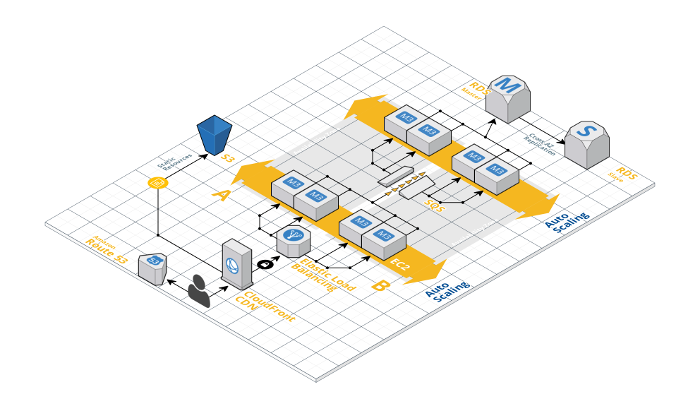
\includegraphics[width=0.8\textwidth]{resources/chapter-2-infrastructure-diagram.png}
        \caption{Contoh gambar}
        \label{fig:1}
    \end{figure}

    \subsubsection{Subsubbab}

    \blindtext
	
	\begin{table}[h!]
		\centering
		\caption{Contoh tabel}
		\begin{tabular}{|c|c|c|c|} 
			\hline
			Col1 & Col2 & Col2 & Col3 \\
			\hline
			1 & 6 & 87837 & 787 \\ 
			\hline
			2 & 7 & 78 & 5415 \\
			\hline
			3 & 545 & 778 & 7507 \\
			\hline
			4 & 545 & 18744 & 7560 \\
			\hline
			5 & 88 & 788 & 6344 \\
			\hline
		\end{tabular}
		\label{table:1}
	\end{table}
	
\section{Studi Terkait}
\blindtext
